\documentclass[12pt,a4paper,oneside,english]{article}
\usepackage[utf8]{inputenc}
\usepackage[T1]{fontenc}
\usepackage{lmodern}
\usepackage[english]{babel}
\usepackage{amsmath}
\usepackage{bm}
\usepackage{xfrac}
\usepackage{a4}
\usepackage{amssymb}
\usepackage{graphicx, caption}
\usepackage[table,xcdraw]{xcolor}
\usepackage{epstopdf}
\usepackage{pgfplotstable}
\usepackage{pgfplots}
\usepackage{siunitx}
\sisetup{separate-uncertainty=true}
\usepackage{tabularx}
\usepackage{booktabs}
\usepackage{varwidth}
\usepackage{float}
\usepackage{german,longtable}
\usepackage{times} % Uncomment to use the Times New Roman font
\setlength\parindent{0pt} % Removes all indentation from paragraphs
\setlength{\parskip}{1em}
\usepackage{gensymb}
\usepackage{listings}
\lstset{basicstyle=\ttfamily\small,breaklines=true}
\usepackage{color,soul}
\usepackage{layouts}
\usepackage{framed}
\colorlet{shadecolor}{gray!25}
\usepackage{hyperref}


% Python style for highlighting
\usepackage{listings}
\DeclareFixedFont{\ttb}{T1}{txtt}{bx}{n}{12} % for bold
\DeclareFixedFont{\ttm}{T1}{txtt}{m}{n}{12}  % for normal
\usepackage{color}
\definecolor{deepblue}{rgb}{0,0,0.5}
\definecolor{deepred}{rgb}{0.6,0,0}
\definecolor{deepgreen}{rgb}{0,0.5,0}
\newcommand\pythonstyle{\lstset{
language=Python,
basicstyle=\ttm,
otherkeywords={self,True,0,1,2,3,4,5,6,7,8,9,False},             % Add keywords here
keywordstyle=\ttb\color{deepblue},
emph={MyClass,__init__},          % Custom highlighting
emphstyle=\ttb\color{deepred},    % Custom highlighting style
stringstyle=\color{deepgreen},
frame=tb,                         % Any extra options here
showstringspaces=false            % 
}}


% Python environment
\lstnewenvironment{python}[1][]
{
\pythonstyle
\lstset{#1}
}
{}

% Python for external files
\newcommand\pythonexternal[2][]{{
\pythonstyle
\lstinputlisting[#1]{#2}}}

% Python for inline
\newcommand\pythoninline[1]{{\pythonstyle\lstinline!#1!}}

\begin{document}
\lstset{language=Python}
	\begin{titlepage}
		\centering
		{\huge\bfseries Designing a particle physics experiment \par}
		\vspace{1cm}
		{\scshape\Large Group project Report\par}
		{Data analysis 2017\par}
		{\today\par}\par
		\vspace{1cm}
		by\par
		\textsc{Stefanie Brühlmeier, Beni Frölich, Dave Linder, Andreas Wiemeyer}
		\vspace{1cm}
		\vspace{1cm}
		supervised by\par
		 \textsc{Michele Atzeni, Arno Gadola, Olaf Steinkamp, Andreas Weiden}
		\vspace{1cm}\par
		\vspace{5cm}
		
\includegraphics[width=0.25\textwidth]{uzh}\par
		\vspace{0.5cm}
		\Large{Physik-Institut der Universität Zürich}
		% Bottom of the page
	\end{titlepage}
	%\maketitle
	\tableofcontents
	\pagebreak
\section{Introduction}
In our project we are dealing with charged kaons which decay exponentially into charged and neutral pions:
\begin{align*}
K^+ \longrightarrow \pi^+ \pi^0
\end{align*}
To simplify the calculations, we neglect the decay of the pions. The aim of this simulation is to determine the distance between a kaon source and a detector which maximizes the acceptance of the detector. The detectors are set up as follows:
\begin{figure}[H]
	\centering
	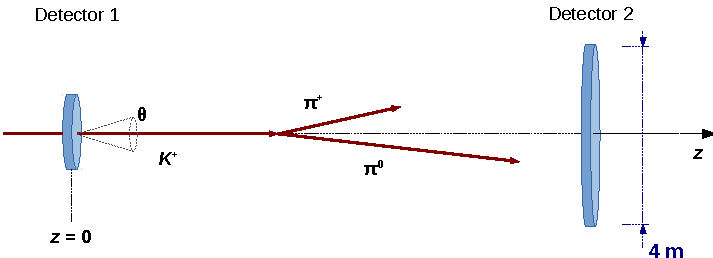
\includegraphics[]{images/setup.pdf}
	\caption{Experimental setup}
	\label{fig:setup}
\end{figure}
As shown in figure \ref{fig:setup} the initial beam of kaons is measured by detector 1 and the resulting pions are measured by detector 2. The second detector is a circular disc with a radius of 2 meters. Depending on 
the location of the decay and
the decay angle (in the $K^+$ rest frame)
the pions might miss the pion detector. Thus, the closer the second detector is to the first, the bigger the probability that the pions are detected. However, if the detector is too close to the first one, the kaons might decay after they have already passed the detector and will therefore not be detected. Given these two constraints, there is a unique optimal distance between the first and the second detector, which we compute with the following simulation. 
In the first part of this project, the average decay length of a $K^+$ is estimated based on a dataset containing the decay lengths of a mix of kaons and pions. Using the result of the first part we can simulate the location of the decay using a Monte-Carlo simulation for an exponential distribution. Further, some impulse vectors\footnote{For the derivation of the isotropic unit vector generator see section \ref{subsec: unit_vector}} (which are distributed isotropically in the $K^+$ rest frame) are generated, supplemented with an energy to form a four-vector and boosted into the laboratory frame. Finally, the percentage of decayed kaons that are detected (called ‘acceptance of the downstream detector’) can be determined. 
The whole simulation is conducted twice, once assuming that the particle beam is parallel to the $z$-axis and once including a Gaussian distributed deviation from the $z$-axis of the particle beam. 
\section{Determination of the average decay length of the $K^+$}
In a first task we should estimate the average decay length of $K^+$ using data of an already conducted experiment in which $100'000$ measurements
of decay lengths $dl_i$ were generated. The particle's beam had a fixed momentum of $\SI{75}{\giga\electronvolt\per\clight}$. However, the beam consisted only of $16\%$ of
$K^+$ . The remaining $84\%$ consisted of $\pi^+$ with a known average decay length of $\beta \gamma c_0 \tau_{\pi^+} = 4.188 \si{\kilo\meter} =
adl_{\pi^+}$.
\begin{figure}[H]
\centering
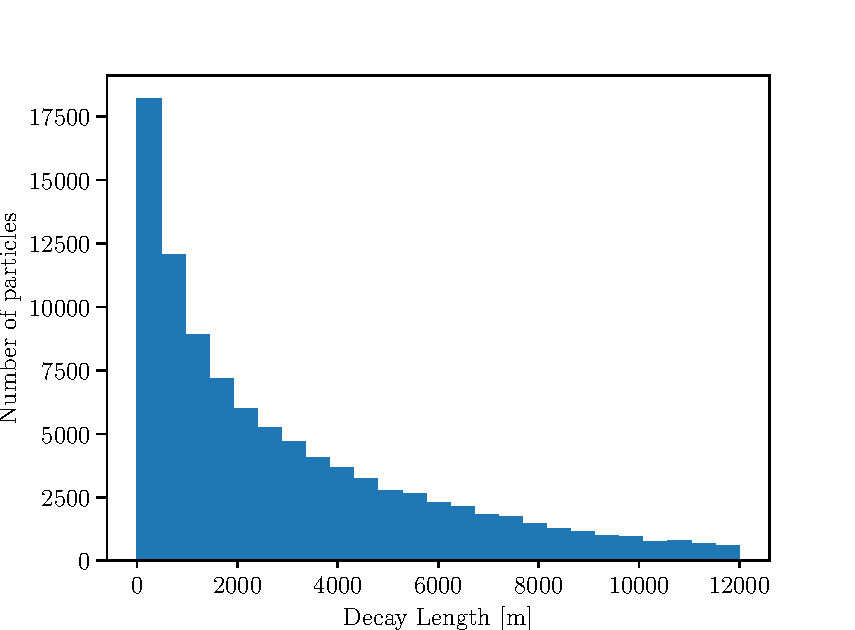
\includegraphics[width=0.8\linewidth]{images/histogram_decay_length.pdf}
	\caption{The particle distribution from a previous experiment with a fixed momentum of $\SI{75}{\giga\electronvolt}$}
	\label{fig:decay}
\end{figure}
To estimate the average decay length of the Kaons $adl_{K^+}$ we used the maximum likelihood method with
the following equation, which was subsequently maximized:
\begin{align}
\ln L(dl_i|adl_{K^+}) = \sum_{i=1}^{N}\ln\left(\frac{0.84}{adl_{\pi^+}}\cdot e^{\frac{-dl_i}{adl_{\pi^+}}}+\frac{0.16}{adl_{K^+}}\cdot e^{\frac{-dl_i}{adl_{K^+}}}\right)
\end{align}
The equation is composed of two exponential distributions, weighted with the corresponding probability that a particle belongs to this distribution. Implementing this in python\footnote{for the python code see appendix in section \ref{subsubse: estimator_code} } resulted in a estimator for the average decay lenght of
\begin{align}
\widehat{adl}_{K^+} = \SI{562(10)}{\meter}
\end{align}
as shown in figure \ref{fig:log_likelihood}
\begin{figure}[H]
\centering
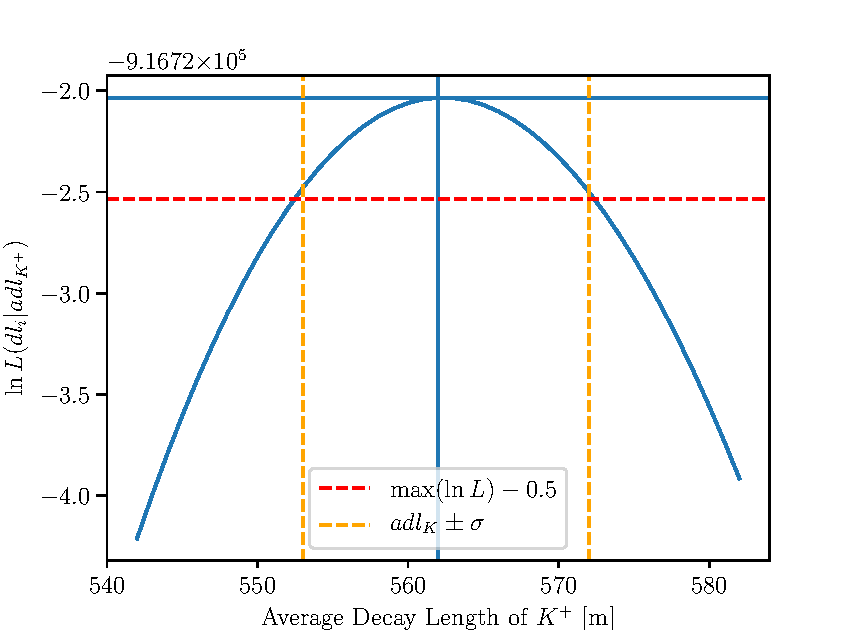
\includegraphics[width=0.8\linewidth]{images/log_likelihood_fuction.pdf}
	\caption{The log-likelihood function around its maximum}
	\label{fig:log_likelihood}
\end{figure}
The error $\sigma_{adl_{K^+}}$ is calculated by
\begin{align}
\ln L(adl_{k^+}\pm\sigma_{adl_{K^+}}) = \ln L(adl_{K^+}) - \frac{1}{2}
\end{align}
Now we can calculate the average decay time
\begin{align}
\tau_{K^+} = \frac{adl_{k^+}}{\beta\gamma c}
\end{align}
Where
\begin{itemize}
	\item $\beta = \frac{|p_k|}{E_K}$
	\item $\gamma = \frac{E_K}{m_K}$
	\item $E = \sqrt{m^2 + |p|^2}$
	\item $|p| = \sqrt{p_x^2 + p_y^2 + p_z^2 } = \SI{75}{\giga\electronvolt\per\clight}$
	\item $m_{K^+} = \SI{493.677(16)e6}{\electronvolt}$\footnote{Found in the following PDF on page 1: http://pdg.lbl.gov/2017/listings/rpp2017-list-K-plus-minus.pdf}
\end{itemize}
Then we get the result
\begin{align}
	\tau_{K^+} = \SI{1.235(22)e-8}{\second}
\end{align}
Compared with the literature value of $\SI{1.2380(20)e-8}{\second}$\footnote{Found in the following PDF on page 2: http://pdg.lbl.gov/2017/listings/rpp2017-list-K-plus-minus.pdf} this result seems reasonable because $\tau_{K^+}$ is within the uncertainty of the pdg value.
\section{Optimal detector distance}
	
We will not follow the order of the exercises from the info sheet, since it is easier to explain our solutions if we look at exercise four and three together. As we will see, exercise three can be solved by simply skipping a step in the solution of exercise four. So what exactly had to be done to solve exercises three and four? The problem can be roughly divided into three parts:
\begin{enumerate}
\item Simulate the path of the kaons from the source to the point where they decay.
\item Calculate the momenta of the pions in the lab frame after the decay.
\item Find the optimal distance by checking how many pions hit the detector for each distance.
\end{enumerate}

1. We can use the results of the first exercise to generate the distance the kaons will travel. For this we use a Monte-Carlo simulation of an exponential decay with a --lambda-- of --1/adl--. Now that we have the distance travelled, we need the direction of flight to determine the location of the decay. For exercise 3 the direction of flight is always along the z-axis, so the locations of the decay can be calculated simply by multiplying the distances travelled with the vector --[0;0;1]--. For exercise 4 we will need to rotate these vectors such that the angles between them and the z-axis match a normal distribution. To do this we generate an angle --alpha-- according to a normal distribution (with a --sigma-- of 1mrad) and a second angle --beta-- according to a uniform distribution (from 0 to --pi--). We then rotate the vectors around the x-axis by --alpha-- and then by --beta-- around the z-axis.
With the first part done we can move on to the second.
	
2. For the calculations done in this part of the simulation we will need (in addition to the list values and equations shown in section 2 of the report) the following list values from the Particle Data Group:

%	MASSEN
	
%	mK+ = (493.677±0.016) * 10**6 eV
%	http://pdg.lbl.gov/2017/listings/rpp2017-list-K-plus-minus.pdf (1)
%	
%	mpi+ = (139.57061±0.00024) * 10**6 eV 
%	http://pdg.lbl.gov/2017/listings/rpp2017-list-pi-plus-minus.pdf (1)
%	
%	mpi0 = (134.9770±0.0005) * 10**6 eV
%	http://pdg.lbl.gov/2017/listings/rpp2017-list-pi-zero.pdf (1)
	
	\begin{align*}
		m_{pi^+ } = \SI{139.5706(24)e6}{\electronvolt}\footnote{Found in the following PDF on page 1: http://pdg.lbl.gov/2017/listings/rpp2017-list-pi-plus-minus.pdf}\\
		m_{pi^0 } = \SI{134.9770(5)e6}{\electronvolt}\footnote{Found in the following PDF on page 1: http://pdg.lbl.gov/2017/listings/rpp2017-list-pi-zero.pdf}\\
	\end{align*}

In the $K^+$ rest frame we now have a momentum of 0 and a rest energy $m_K^+$. The $K^+$ now decays into a $\pi^+$ and a $\pi^0$ with momenta $p_{\pi^+} $, $p_{\pi^0} $ in oposing directions. The momenta must have the same magnitude and $p_{\pi^+} = -p_{\pi^0} $ .
	
The magnitude of the momentum is calculated with the energy of lost mass in the decay. In the following equations $p$ is used as absolute scalar.
		
	\begin{align}
		E_{\pi^+} = \frac{m_{K^+}^2 + m_{pi^+ }^2 - m_{pi^0 }^2 } {2 m_{K^+}}\\
		p_{\pi^+} = \sqrt{E_{\pi^+}^2 - m_{pi^+ }^2 }\\
		p_{\pi^+ } = p_{\pi^0 }\\
	\end{align}
	
We use isotropically distributed unit vectors in the simulation (see Appendix A.1). We multiply them with $p_{\pi^0}$ to get the momenta for $\pi^0$ in the $K^+$ rest frame. To get the momenta of $\pi^+$ we take the same distribution and flip signs. We then build the four vectors  $P^*_{\pi}$.
	
	\begin{align}
		 P^*_{\pi} = 
		\begin{bmatrix}
				E_{\pi}^* \\ p_{\pi,x}^* \\ p_{\pi,y}^* \\ p_{\pi,z}^*
		\end{bmatrix} = 
		\begin{bmatrix}
				\sqrt{m_{\pi}^2 + ||p_{\pi}||^2 } \\ p_{\pi,x}^* \\ p_{\pi,y}^* \\ p_{\pi,z}^*
		\end{bmatrix}
	\end{align}
	
Back to the lab rest frame, we boost them with the boost matrix. This boost matrix performs a boost along the z-axis. 
	
	\begin{align}
		P_{\pi} =
		\begin{bmatrix}
		\gamma & 0 & 0 & \beta \gamma \\
		0 & 1 & 0 & 0 \\
		0 & 0 & 1 & 0\\
		\beta \gamma & 0 & 0 & \gamma \\
		\end{bmatrix}
		\cdot
		P^*_{\pi}
	\end{align}
	
$P_{\pi}$ is the four-vector in the lab frame. $P_{\pi}^*$ is the four-vector in the kaon rest frame. So much for the beam of kaons that is perfectly alligned with the z-axis. Now to the slighly more complicated part.
	
\subsection{With scattering}

When we use a beam that is not parallel to the z-axis, we need to perform a rotation to the momentum of the four-vector before and after the boost. The rotation after the boost is the same that would rotate $e_z$ to align with the position vector. The one before is the inverse rotation.
		
%Since the momentum of the four-vectors $P_{\pi}$ of the pions are isotropically distributed in the  $K^+$ rest frame, we can omit the first rotation and still end up with a an isotropical distribution.%
		
The operation performed with the angle $\alpha$ around y-axis and $\beta$ around x-axis:
		
		\begin{align}
				R(\alpha, \beta) = \begin{bmatrix}
				\cos \alpha  & 0 & \sin \alpha \\
				0         & 1 &  0          \\
				-\sin \alpha & 0 & \cos \alpha
				\end{bmatrix} \cdot \begin{bmatrix}
				1 &   0         & 0           \\
				0 & \cos \beta & -\sin \beta \\
				0 & \sin \beta &  \cos \beta
				\end{bmatrix}
		\end{align}
		
We apply $R(\alpha, \beta)$ to the momentum after we have extracted	the momentum of the four-vector $P_{\pi}$.
		
\subsection{Counting double hits}
\label{hits}
		
To determine the number of decays for which both pions hit the detector, we first define its position on the z-axis $z_d$ and its radius $r$. The impulses in the lab frame are $\overrightarrow{p_{\pi^+}}$ and $\overrightarrow{p_{\pi^0}}$. The decay position are given by $\overrightarrow{x} = (x, y, z)$. To find the number of double hits we perform the following steps\footnote{See Appendix \ref{subsubse: single_hit_code} for single hits and \ref{subsubse: double_hit_code} for double hits implementation in Python}:
				
		\begin{enumerate}
			\item Disregard all the decays where $z > z_d$.
			\item Do the following for $\overrightarrow{p} = \overrightarrow{p_{\pi^+}}$ or $\overrightarrow{p_{\pi^0}}$.
			\begin{enumerate}
				\item Calculate the point of intersection $\overrightarrow{q}$ of $\overrightarrow{p}$ and the plane orthogonal to the z-axis at $z_d$ (the plane in which the detector lies).
				\item Disregard the pion if $\overrightarrow{q}$ lies outside of the detector, that is $ (x + q_x)^2 + (y + q_y)^2 > r^2$. % code 1
			\end{enumerate}
			\item Disregard the decay if one of the two pions was disregarded.
			\item Count the number of decays left. % code  2
		\end{enumerate}
	
	% code 1 TODO: reference code file...
%
	
		% code 2
%		def count_double_hits(decay_positions, particle1_4vec, particle2_4vec, r, z_detector):
%		"""count for how many of the decays, particle1 and particle2 hit the detector"""
%		
%		# numpy filter to filter the ones that decay in front of the detector
%		in_front = decay_positions[:,2] < z_detector
%		
%		# drop the decays that are behind
%		decay_positions = decay_positions[in_front]
%		particle1_4vec = particle1_4vec[in_front]
%		particle2_4vec = particle2_4vec[in_front]
%		
%		# boolean array. True if hit, False if miss
%		hits1 = single_hit(decay_positions, particle1_4vec, z_detector, r)
%		hits2 = single_hit(decay_positions, particle2_4vec, z_detector, r)
%		
%		# combine the with elementwise and.
%		hits = hits1 & hits2
%		return len(decay_positions[hits])

	
\subsection{Determine optimal detector distance $z_d$}
We will now determine the distance between the source and the detector where the acceptance of the detector is maximized. We will call this distance the optimal distance. Before we can do this we need to define what is meant by the acceptance P of the detector:
	
	\begin{align}
		P(z_d) = \frac{\text{$n$ decays for which both pions hit at $z_d$}}{\text{$n$ decays simulated}} 
	\end{align}
	
To maximize this acceptance we run the experiment about 500 times with $N = 10^6 $ kaons generated. First we simulate a beam aligned to the $z$-axis. Second we generate a beam that scatters at the source in a gaussian distribution with $\sigma _{\theta} = 0.001$ rad (see previous sections). 
	
To determine the optimal $z$-distance, we implemented the algorithm described in \ref{hits}. We let it run for z values in a range from 215 to 350 meters in 85 evenly sized steps. The algorithm generates 85 double hit counts in an array. We divide by N to get the acceptance of the respective $z$-distance. Then we plot the acceptance as a function of the $z$-distance, fit it with a third degree polynomial and determine the maximum of that polynomial. The simulation was run once with $N = 10^6 $ decays.
	
\begin{figure}
	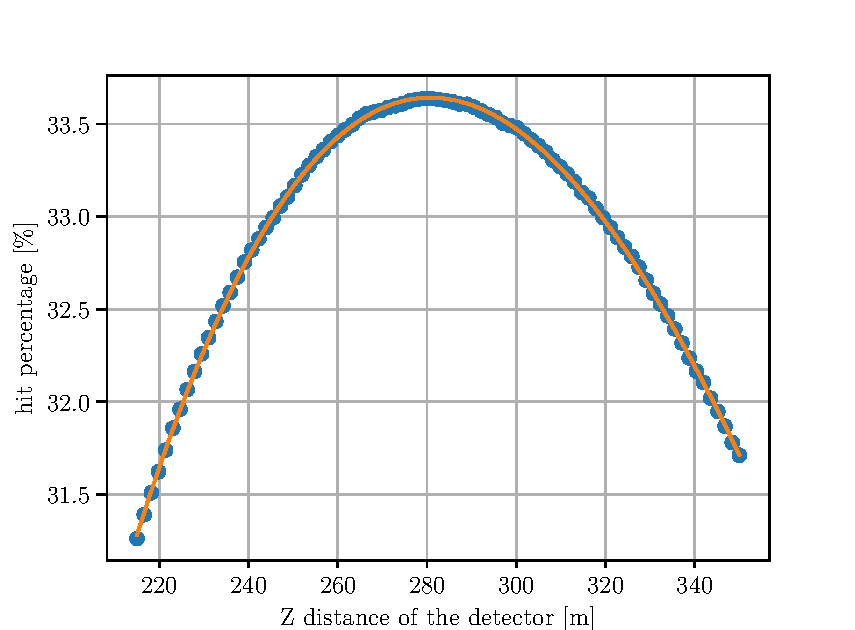
\includegraphics[width=\linewidth]{images/sample_figure_1000000.pdf}
	\caption{Sample output of decay\_simulation\_optimized.py}
	\label{fig:figure1000000215to350in85562}
\end{figure}
	
We run the simulation about 500 times. Fitting the maximum and saving it. The maxima are then put into a histogram. The averages and standard deviations of the maxima are listed below. The standard deviation gives a measure of the statistical uncertainty on the optimal distance.
	
	%[TODO add units]% 
	
	\textbf{Results for the aligned Beam:}
		\begin{align*}
		z = \SI{285.5}{\meter}\\
		\sigma _z  : \SI{0.7}{\meter}\\
		\end{align*}
	
	\textbf{Results for the Scattered Beam:}
		\begin{align*}
		z = \SI{280.7}{\meter}\\
		\sigma _z  : \SI{0.7}{\meter}\\
		\end{align*}
		
To calculate the final uncertainty we used the relative error on the average decay length from chapter [TODO add reference]. The relative errors get quadratically added.
		
		\begin{align}
			m_z = \sigma _z \cdot \sqrt{ \left(\frac{\text{uncertanty on adl}}{\text{adl}}\right)^2 +  \left(\frac{\sigma_z}{z}\right)^2}
		\end{align}
		
		The final optimal values for z are:
		
		\begin{align*}
			z_{\text{aligned}} =  \SI{286(5)}{\meter}\\
			z_{\text{scattered}} =  \SI{281(5)}{\meter}
		\end{align*}
		
		The error does not matter that much, since a change of $5$ meters around the maximum does maximally change the acceptance by $0.5\%$ as seen in figure \ref{fig:figure1000000215to350in85562}.
		
\begin{figure}[H]
	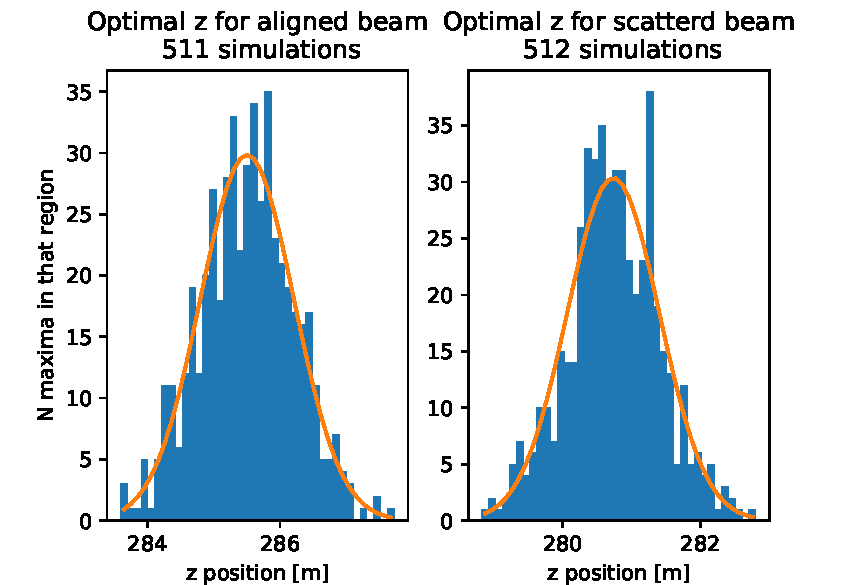
\includegraphics[scale=1]{images/optimal_zpos.pdf}
	\caption{The histogrammed results of the simulations and their gaussian fits (l: aligned, r: scattered)}
	\label{fig:optimalzpos}
\end{figure}

\section{Conclusion}
If we were to account for pion decay the optimal distance would be shorter.
\appendix
\section{Appendix}
\subsection{Derivation of the isotropic unit vector generator}
\label{subsec: unit_vector}
For exercise 3 we need to generate vectors that are isotropically distributed in three-dimensional space. That is, we need to generate vectors that have an equal chance to point in any direction. This is not as simple as calculating two uniformly distributed angles phi and psi and rotating a vector around two different axes by these angles. To see this one can do the following:

Imagine a sphere whose centre is, for sake of simplicity, situated at the centre of the coordinate system and whose radius is one. Now imagine a vector that reaches from its centre to its surface. Again, for sake of simplicity, let’s say that this vector is aligned with one axis (let’s say the $z$-axis to match our code). We are interested in the position of the end-point of the vector. The vector is now rotated by $\phi$ along one axis orthogonal to its starting position (say the $x$-axis) and then rotated again by psi around the other axis orthogonal to its starting position (the $y$-axis). We can see that the first rotation determines a limited space through which the end-point can move by rotating the vector around the $y$-axis. More precisely, this space is a circle on the surface of the sphere with its centre on the $y$-axis. The probability $p$ of the angle corresponding to each of these circles will determine how probable it is to have the end-point land somewhere on them. Since the distribution is supposed to be isotropical, we want the probability for the end-point to land on any point of the circle to be constant.
\begin{figure}[H]
	\centering
	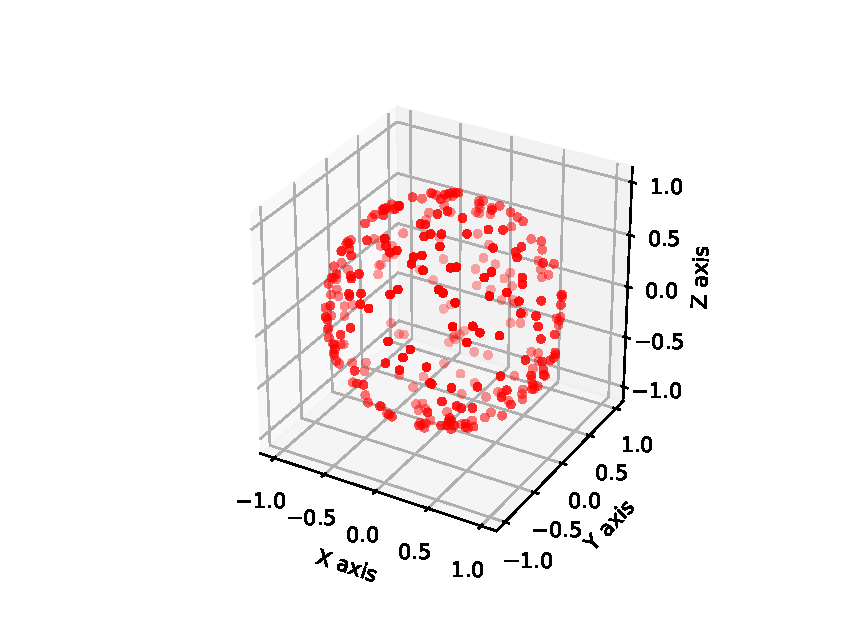
\includegraphics[width=0.7\linewidth]{images/three_vector.pdf}
	\caption{Randomly distributed three vector on a unit sphere.}
	\label{fig:threevec}
\end{figure}
From this follows that the probability to land on each circle should be proportional to its circumference. Since the circumference of the circle is a non-constant function of $\phi$ and since (as we have stated) the probability to land on one circle is equal to the probability of the corresponding $\phi$, the probability for all angles $\phi$ mustn’t be constant. We can calculate the probability for each angle as follows:
\begin{align}
p(\phi) \propto \text{circumference} \implies \frac{p(\phi)}{\text{circumference}} = k \quad  k \in \mathbb{R}
\end{align}
And the circumference is given by the following equation:
\begin{align}
\text{circumference} = 2  \pi \cdot \cos(\phi)
\end{align}
Using this we get an equation for $p(\phi)$:
\begin{align}
\frac{p(\phi)}{2\pi\cdot \cos(\phi)} = k \Longleftrightarrow p(\phi) = k \cdot 2\pi \cdot \cos(\phi)
\end{align}
Since $\phi \in (\frac{-\pi}{2}, \frac{\pi}{2}]$ we want the function to be normalized over this range:
\begin{align}
\int_{-\pi/2}^{\pi/2}k\cdot 2\pi \cdot \cos(\phi) \overset{!}{=} 1 \implies k \cdot 4\pi  = 1 \implies k = \frac{1}{4\pi}
\end{align}
And we get the final equation:
\begin{align}
p(\phi) = \frac{1}{2}\cos(\phi)
\end{align}
Now we need to somehow get a value between $(\frac{-\pi}{2}, \frac{\pi}{2}]$ that is distributed according to this function implemented in python. We weren’t aware of a built-in function for this job, so we needed to get there on our own, using a uniform distribution as a starting point. To make our solution evident one can do the following.
Think of the area under the probability curve $p(\phi)$. If we scatter dots evenly across this area, the amount of dots under an infinitely small segment of the curve will be proportional to the area under the curve and thus the value of the curve at the segment. In other words: the amount of dots under the curve at $\phi$ will be proportional to $p(\phi)$. Now Imagine the Integral of the probability curve $p(\phi)$ as a sum of thin slices. Instead of having the pillars standing next to each other in the graph, imagine stacking them on top of each other. The leftmost pillar at the bottom, the rightmost pillar at the top. The scattered dots would now be uniformly distributed across the height of the stacked pillars. We can generate this distribution. All we need is a function to calculate back from the height in the stack to the angle $\phi$.
To find this function we take the Integral of $p(\phi)$ from $-\pi/2$ to an undetermined value $a \in (-\frac{\pi}{2}, \frac{pi}{2}]$:
\begin{align}
\int_{-\pi/2}^{a}\frac{1}{2}\cos(\phi) = \frac{1}{2} \sin(\phi) \bigg|_{-\pi/2}^{a} = \frac{\sin(a)+1}{2}
\end{align}
Speaking in our previous pseudomathematic language, this function assigns a height in the stack of pillars to any value $a$. The absolute height of the pillar is unimportant for this to work. All we need to insure is that the range of the uniformly distributed values is equal to the range of the integral. Since the Integral ranges from $0$ to $1$, we will uniformly distribute from $0$ to $1$ as well. Now we just need to invert the previous Integral to get the function we were looking for.
\begin{align}
y = \frac{\sin(a)+1}{2} \implies a=\arcsin(2y-1)
\end{align}
With $y$ being uniformly distributed values from $0$ to $1$ we can use this equation to get the correct $\phi(a)$. Now all that’s left to do is to rotate the vector $[0;0;1]$ first by $\phi$ around the $x$-axis and then by $\psi$ around the $y$-axis.
\subsection{Python code}
\subsubsection{Implementing of the weighted exponential distributions to compute the estimator $\widehat{adl}_{K^+}$}
\label{subsubse: estimator_code}
\begin{shaded}
\begin{python}
def f(length, length_K):
    return np.log((0.16/ length_K) * np.exp(-length / length_K) + (0.84/ length_pi) * np.exp(-length/ length_pi))

def ll(length_K):
    total = 0
    for length in lengths:
        total += f(length, length_K)
    return total

LLs = ll(length_Ks)

length_K_hut = length_Ks[list(LLs).index(max(LLs))]
\end{python}
\end{shaded}
\subsubsection{Implementation of the single\_hit function}
\label{subsubse: single_hit_code}
\begin{shaded}
	\begin{python}
def single_hit(decay_position, four_vecs, z_detector, detector_radius):
"""check if one particle hit the detector"""
	p = four_vecs[:, 1:]
	x, y, z = decay_position.T
	
	# q is the position the particle will pass in the plane through z_detector
	q = p.T * (-z + z_detector) / p[:,2]
	qx, qy, qz = q
	
	# return whether the particles hit the circular disk
	return (x + qx)**2 + (y + qy)**2 < detector_radius**2
	
		\end{python}
\end{shaded}


\subsubsection{Implementation of the count\_double\_hits function}
\label{subsubse: double_hit_code}
\begin{shaded}
	\begin{python}
def count_double_hits(decay_positions, particle1_4vec, particle2_4vec, r, z_detector):
	"""count for how many of the decays, particle1 and particle2 hit the detector"""
	
	# numpy filter to filter the ones that decay in front of the detector
	in_front = decay_positions[:,2] < z_detector
	
	# drop the decays that are behind
	decay_positions = decay_positions[in_front]
	particle1_4vec = particle1_4vec[in_front]
	particle2_4vec = particle2_4vec[in_front]
	
	# boolean array. True if hit, False if miss
	hits1 = single_hit(decay_positions, particle1_4vec, z_detector, r)
	hits2 = single_hit(decay_positions, particle2_4vec, z_detector, r)
	
	# combine the with elementwise and.
	hits = hits1 & hits2
	return len(decay_positions[hits])

	\end{python}
\end{shaded}

	
\end{document}